\documentclass[../../main.tex]{subfiles}

\begin{document}
\section{Riprogettazione proposta}
In questa sezione, descriviamo gli aspetti salienti dell'interfaccia frutto della nostra riprogettazione ed evidenziamo gli accorgimenti adottati per risolvere le criticità discusse in \hyperref[s:considerazioni]{Sezione 2 Considerazioni sulla dashboard del DPC}, nonché le funzionalità aggiunte per concorrere ad una esperienza utente piacevole e produttiva.

Ancor prima di addentrarci nella trattazione, spendiamo qualche riga per parlare del lungo e  rigoroso processo tramite cui abbiamo dato forma alla nostra riprogettazione:
\begin{enumerate}
    \item \textbf{Ricerca etnografica}: abbiamo definito il segmento etnografico cui intendiamo fornire supporto, rinvenendolo nei giornalisti che pubblicano articoli sull'andamento di vari aspetti quantitativi della pandemia (contagi giornalieri, decessi, guariti, tamponi, occupazione delle terapie intensive, ricoveri...), non necessariamente con background scientifico (liceo scientifico, Scienze matematiche, fisiche e naturali (in sigla MM.FF.NN.)).
    \item \textbf{Verifica delle risorse esistenti}: abbiamo valutato le dashboard esistenti in termini di una lunga serie di linee guida riconosciute, così da comprenderne i margini di miglioramento, nonché i punti di forza; ci siamo rivolti a svariati giornalisti affinché testassero le interfacce esistenti, al fine di avere evidenza di quanto riscontrato nella valutazione precedente;
    \item \textbf{Studio di fattibilità}: abbiamo definito il contesto in cui sono fruite le dashboard informative sul Covid-19;
    \item \textbf{Proposta di design}: abbiamo seguito il modello CAO=S e condotto studi circa l'architettura delle informazioni e la modalità di interazione, così da raccogliere tutti gli ingredienti essenziali per un'usabilità elevata e un'esperienza d'uso soddisfacente; abbiamo dato  loro forma mediante un blueprint e vari wireframe;
    \item \textbf{Valutazione del design}: abbiamo condotto ben due tipologie di testing sull'interfaccia da noi riprogettata; nella prima abbiamo valutato nuovamente le linee guida di cui al punto 2, mentre nella seconda ci siamo rivolti a giornalisti per averne opinioni e impressioni;
\end{enumerate}

\clearpage
\section{Descrizione dell'interfaccia}
L'interfaccia risultante dalla nostra riprogettazione appare strutturata in quattro differenti schermate, tra cui l'utente può navigare liberamente: nei paragrafi che seguono forniamo una descrizione di ognuna, evidenziando come riescano ad ampliare il portato informativo eccessivamente limitato dell'interfaccia originaria, come discusso in \hyperref[ss:criticita-informative]{Sezione 2.2 Criticità nella capacità informativa}.

\subsection{Panoramica}
\begin{figure}[h]
    \centering
    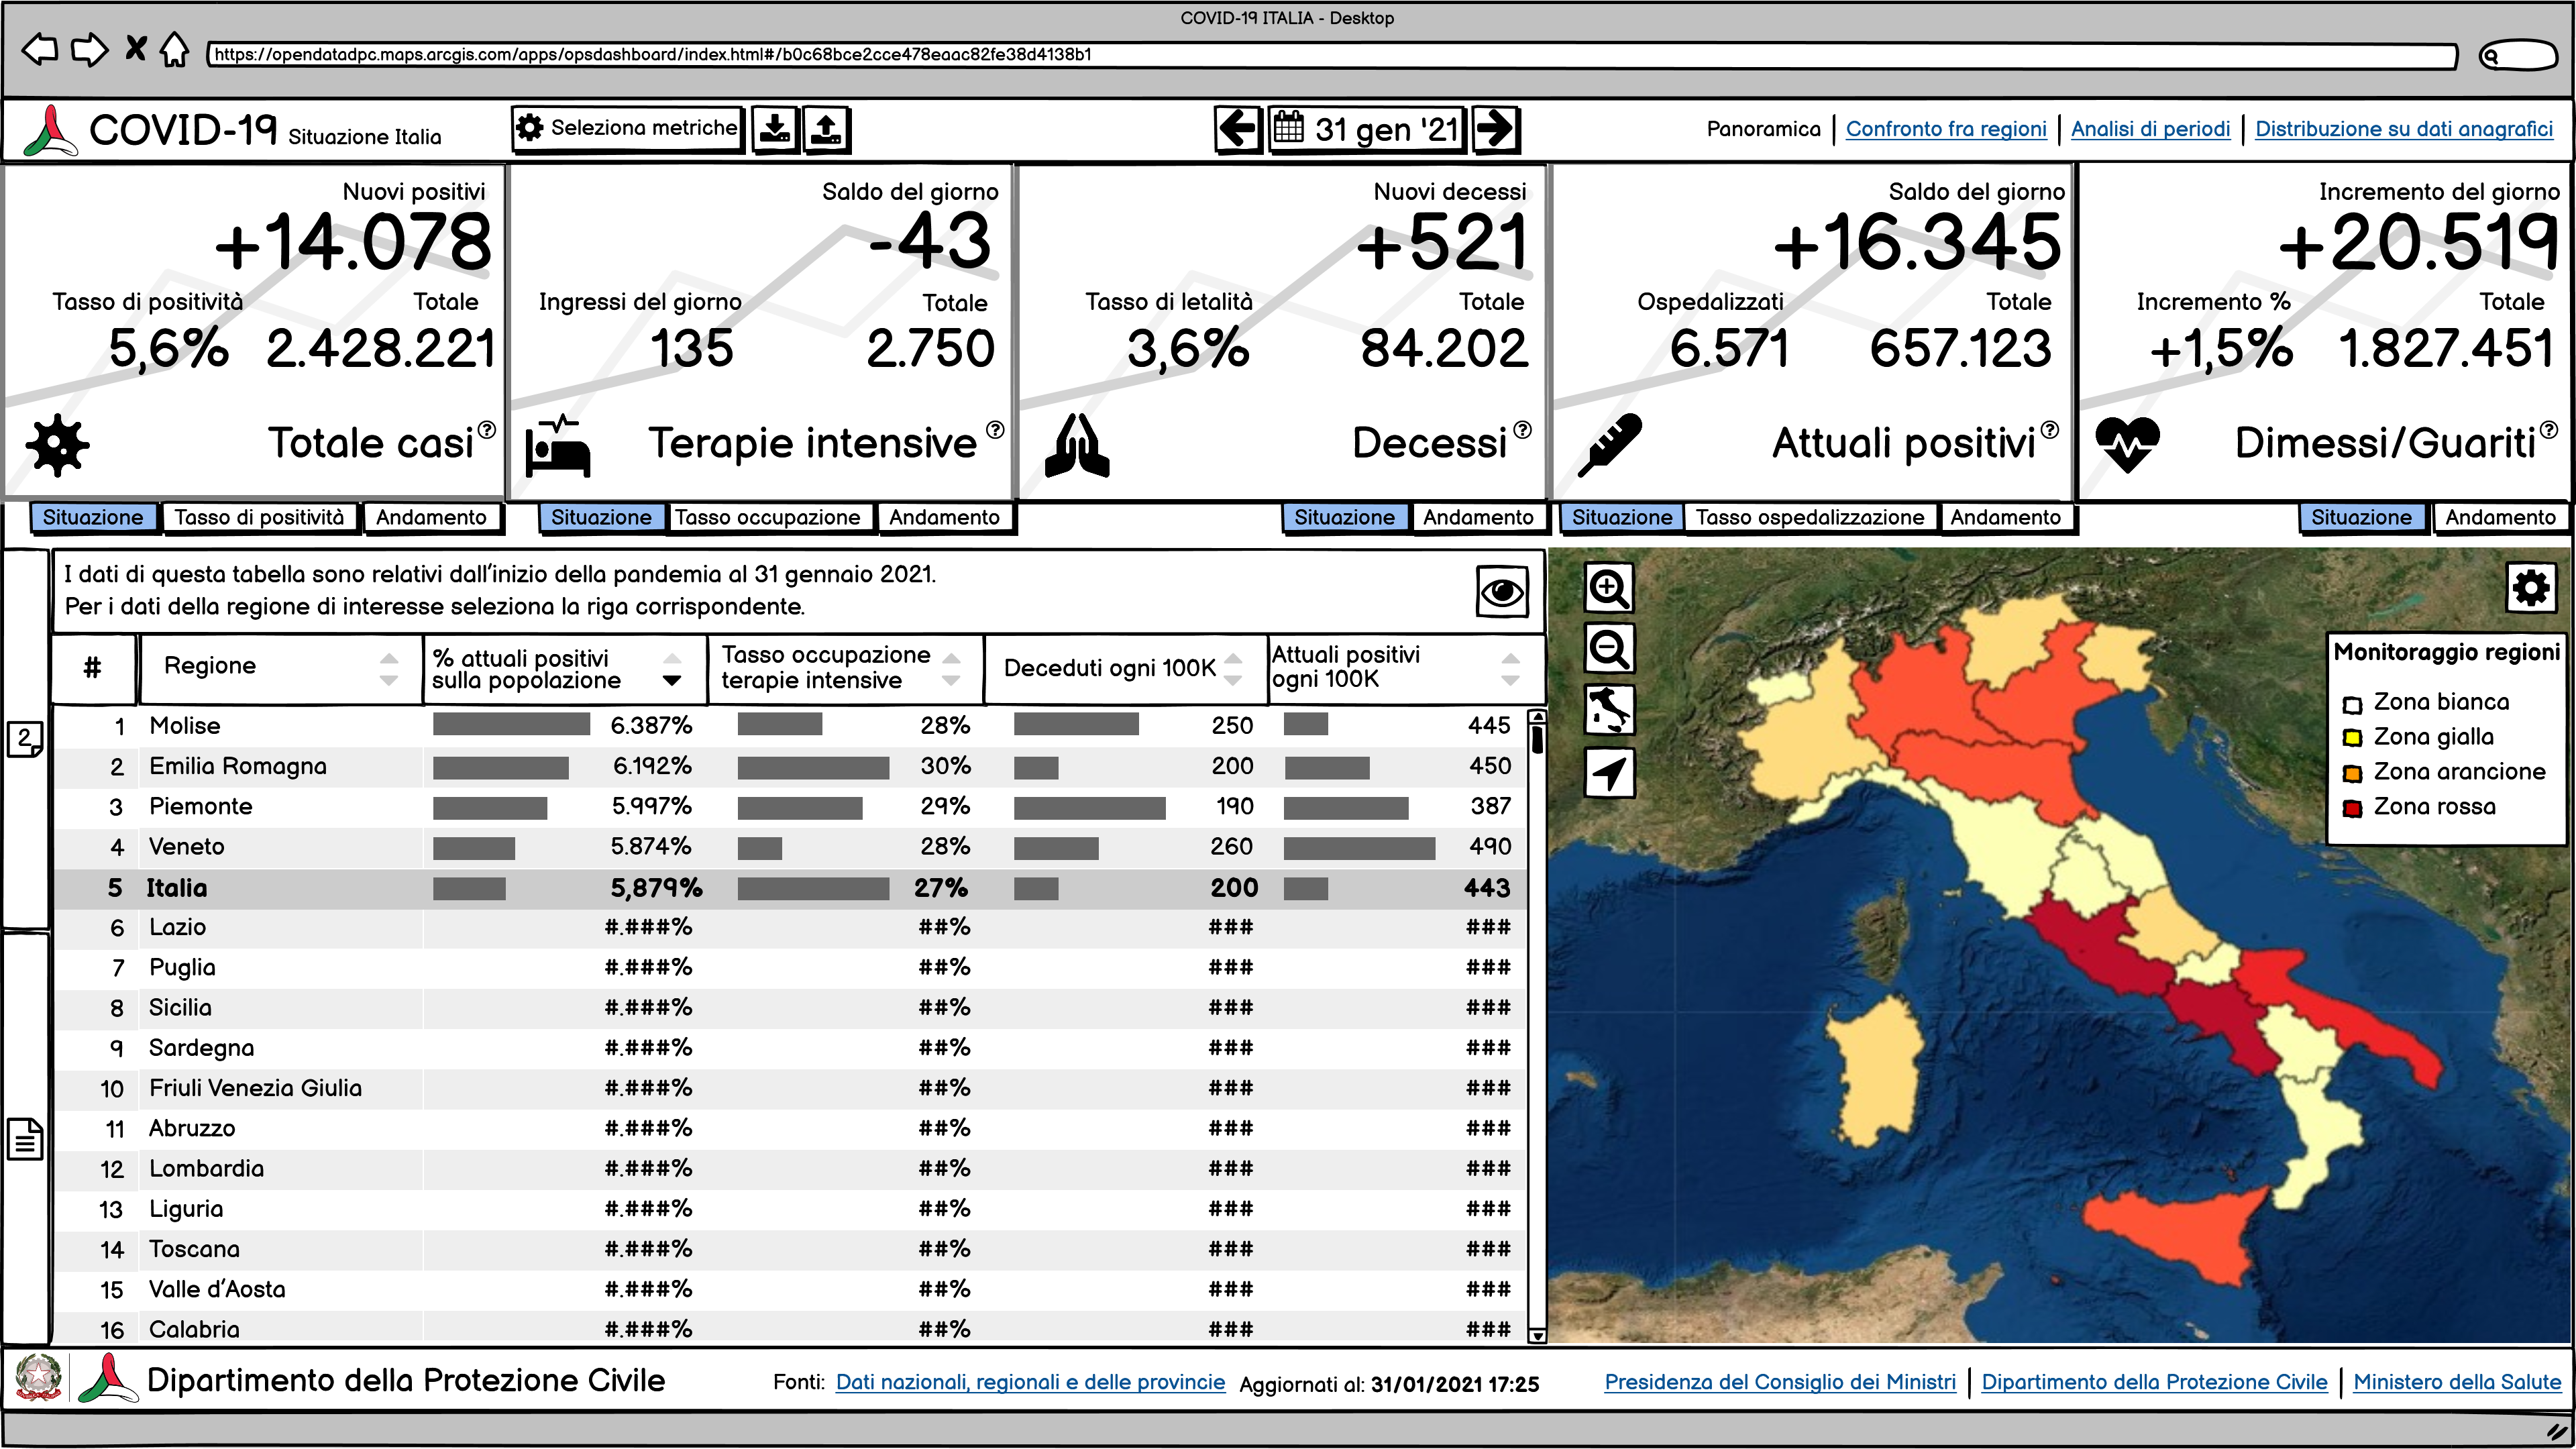
\includegraphics[width = \textwidth]{../img/1 - Panoramica}
    \caption{Schermata "Panoramica" dell'interfaccia riprogettata.}
    \label{fig:panoramica}
\end{figure}

Questa schermata, come suggerito chiaramente dal nome, presenta all'utente una panoramica dei valori delle metriche epidemiologiche ritenute fondamentali in base a quanto emerso dall'ascolto dei giornalisti.\\
In dettaglio, la parte superiore visualizza dei box, ciascuno dei quali presenta delle schede selezionabili: in linea generale, in essi il giornalista potrà leggere i totali delle metriche suddette e le loro variazioni rispetto al giorno precedente a quello specificato, nonché indicatori di livello o curve del loro andamento nel periodo temporale indicato mediante gli slider.\\

Nella parte inferiore, l'utente può interagire con una tabella che presenta i dati epidemiologici per le regioni italiane; ancora, vi è una heat map che offre un efficace colpo d'occhio circa la distribuzione della metrica selezionata sul territorio nazionale. L'utente può richiedere alla dashboard che gli siano restituiti i dati relativi ad una specifica regione cliccando sulla sua area nella mappa oppure sulla riga corrispondente della tabella.

\clearpage
\subsection{Confronto fra regioni}
\begin{figure}[h]
    \centering
    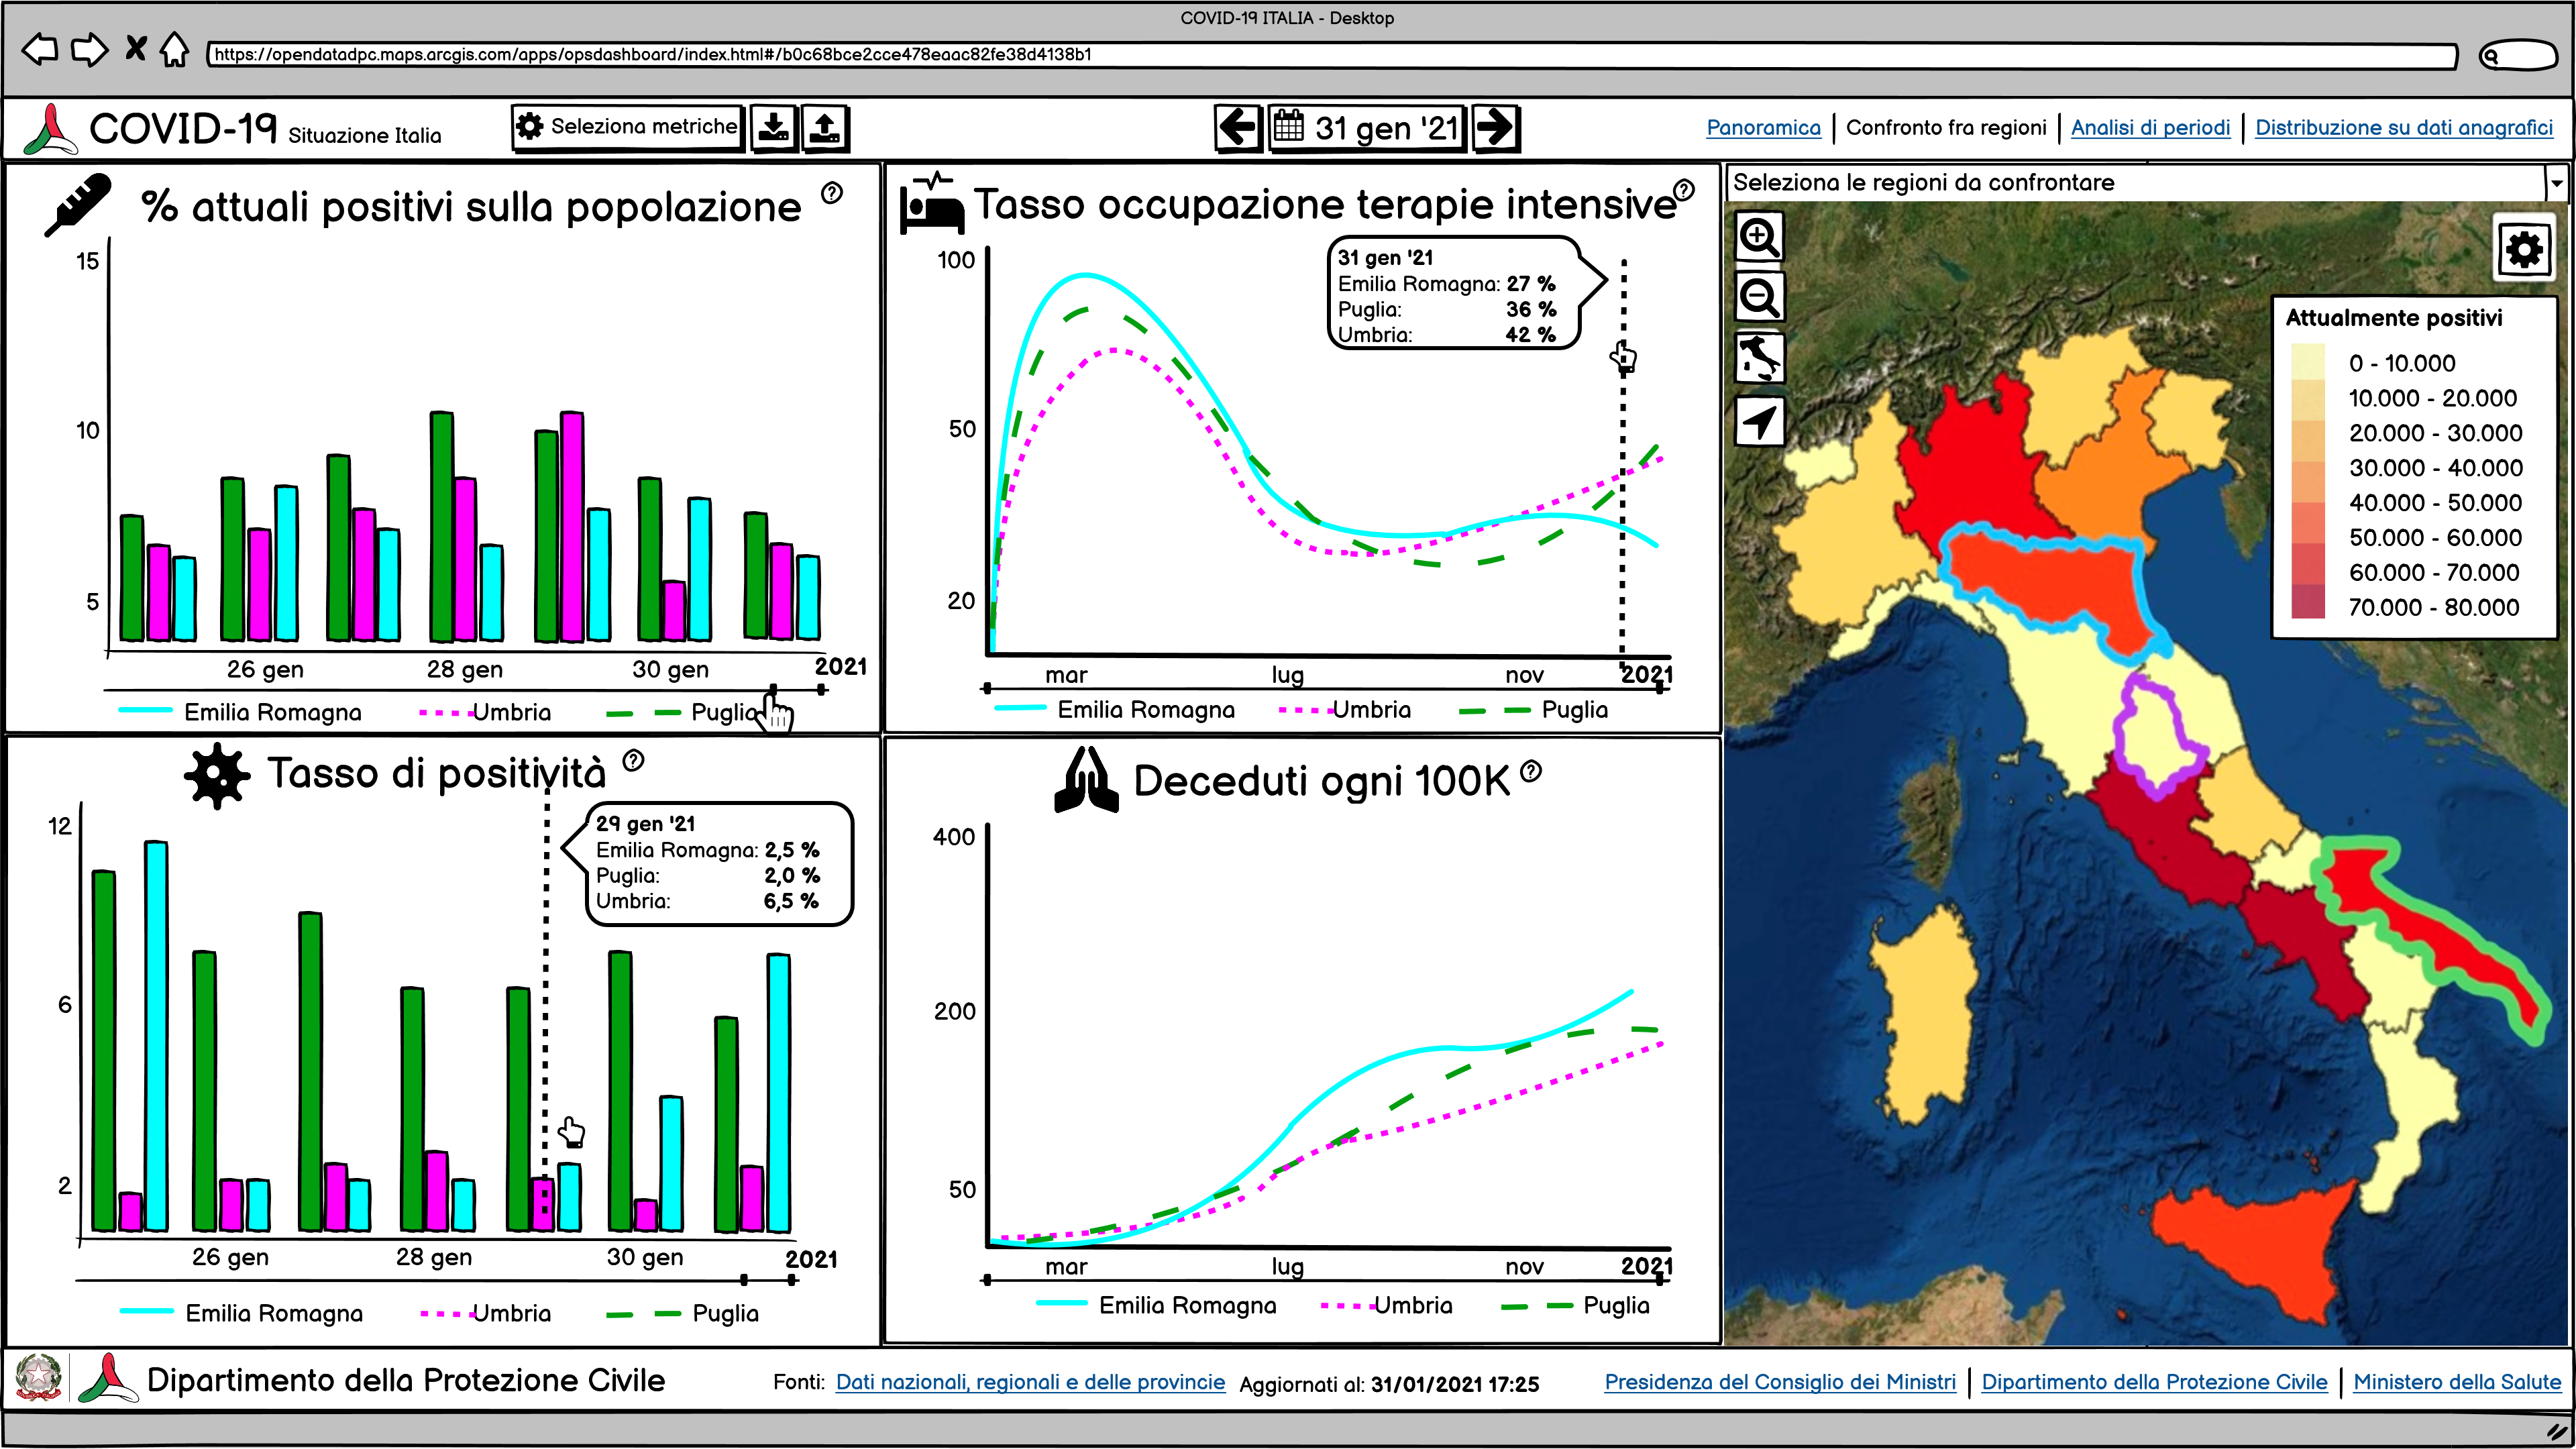
\includegraphics[width = \textwidth]{../img/1 - Confronto fra regioni}
    \caption{Schermata "Confronto tra regioni" dell'interfaccia riprogettata.}
    \label{fig:confronto-regioni}
\end{figure}
La schermata in oggetto è particolarmente significativa qualora i giornalisti intendano confrontare il quadro epidemiologico tra due o più regioni: essi possono selezionare direttamente sulla mappa l'area delle regioni di loro interesse ovvero cliccarvi nell'elenco a discesa subito sopra la mappa stessa. A seguito di questa sua interazione, ecco che sulla parte sinistra dell'interfaccia, quattro grafici si popolano con i dati relativi alle regioni specificate: in questa maniera, i giornalisti possono condurre agevolmente un confronto dell'andamento delle metriche nelle regioni, entro un'unica e omogenea esperienza utente.
\clearpage
\subsection{Analisi di periodi}
\begin{figure}[h]
    \centering
    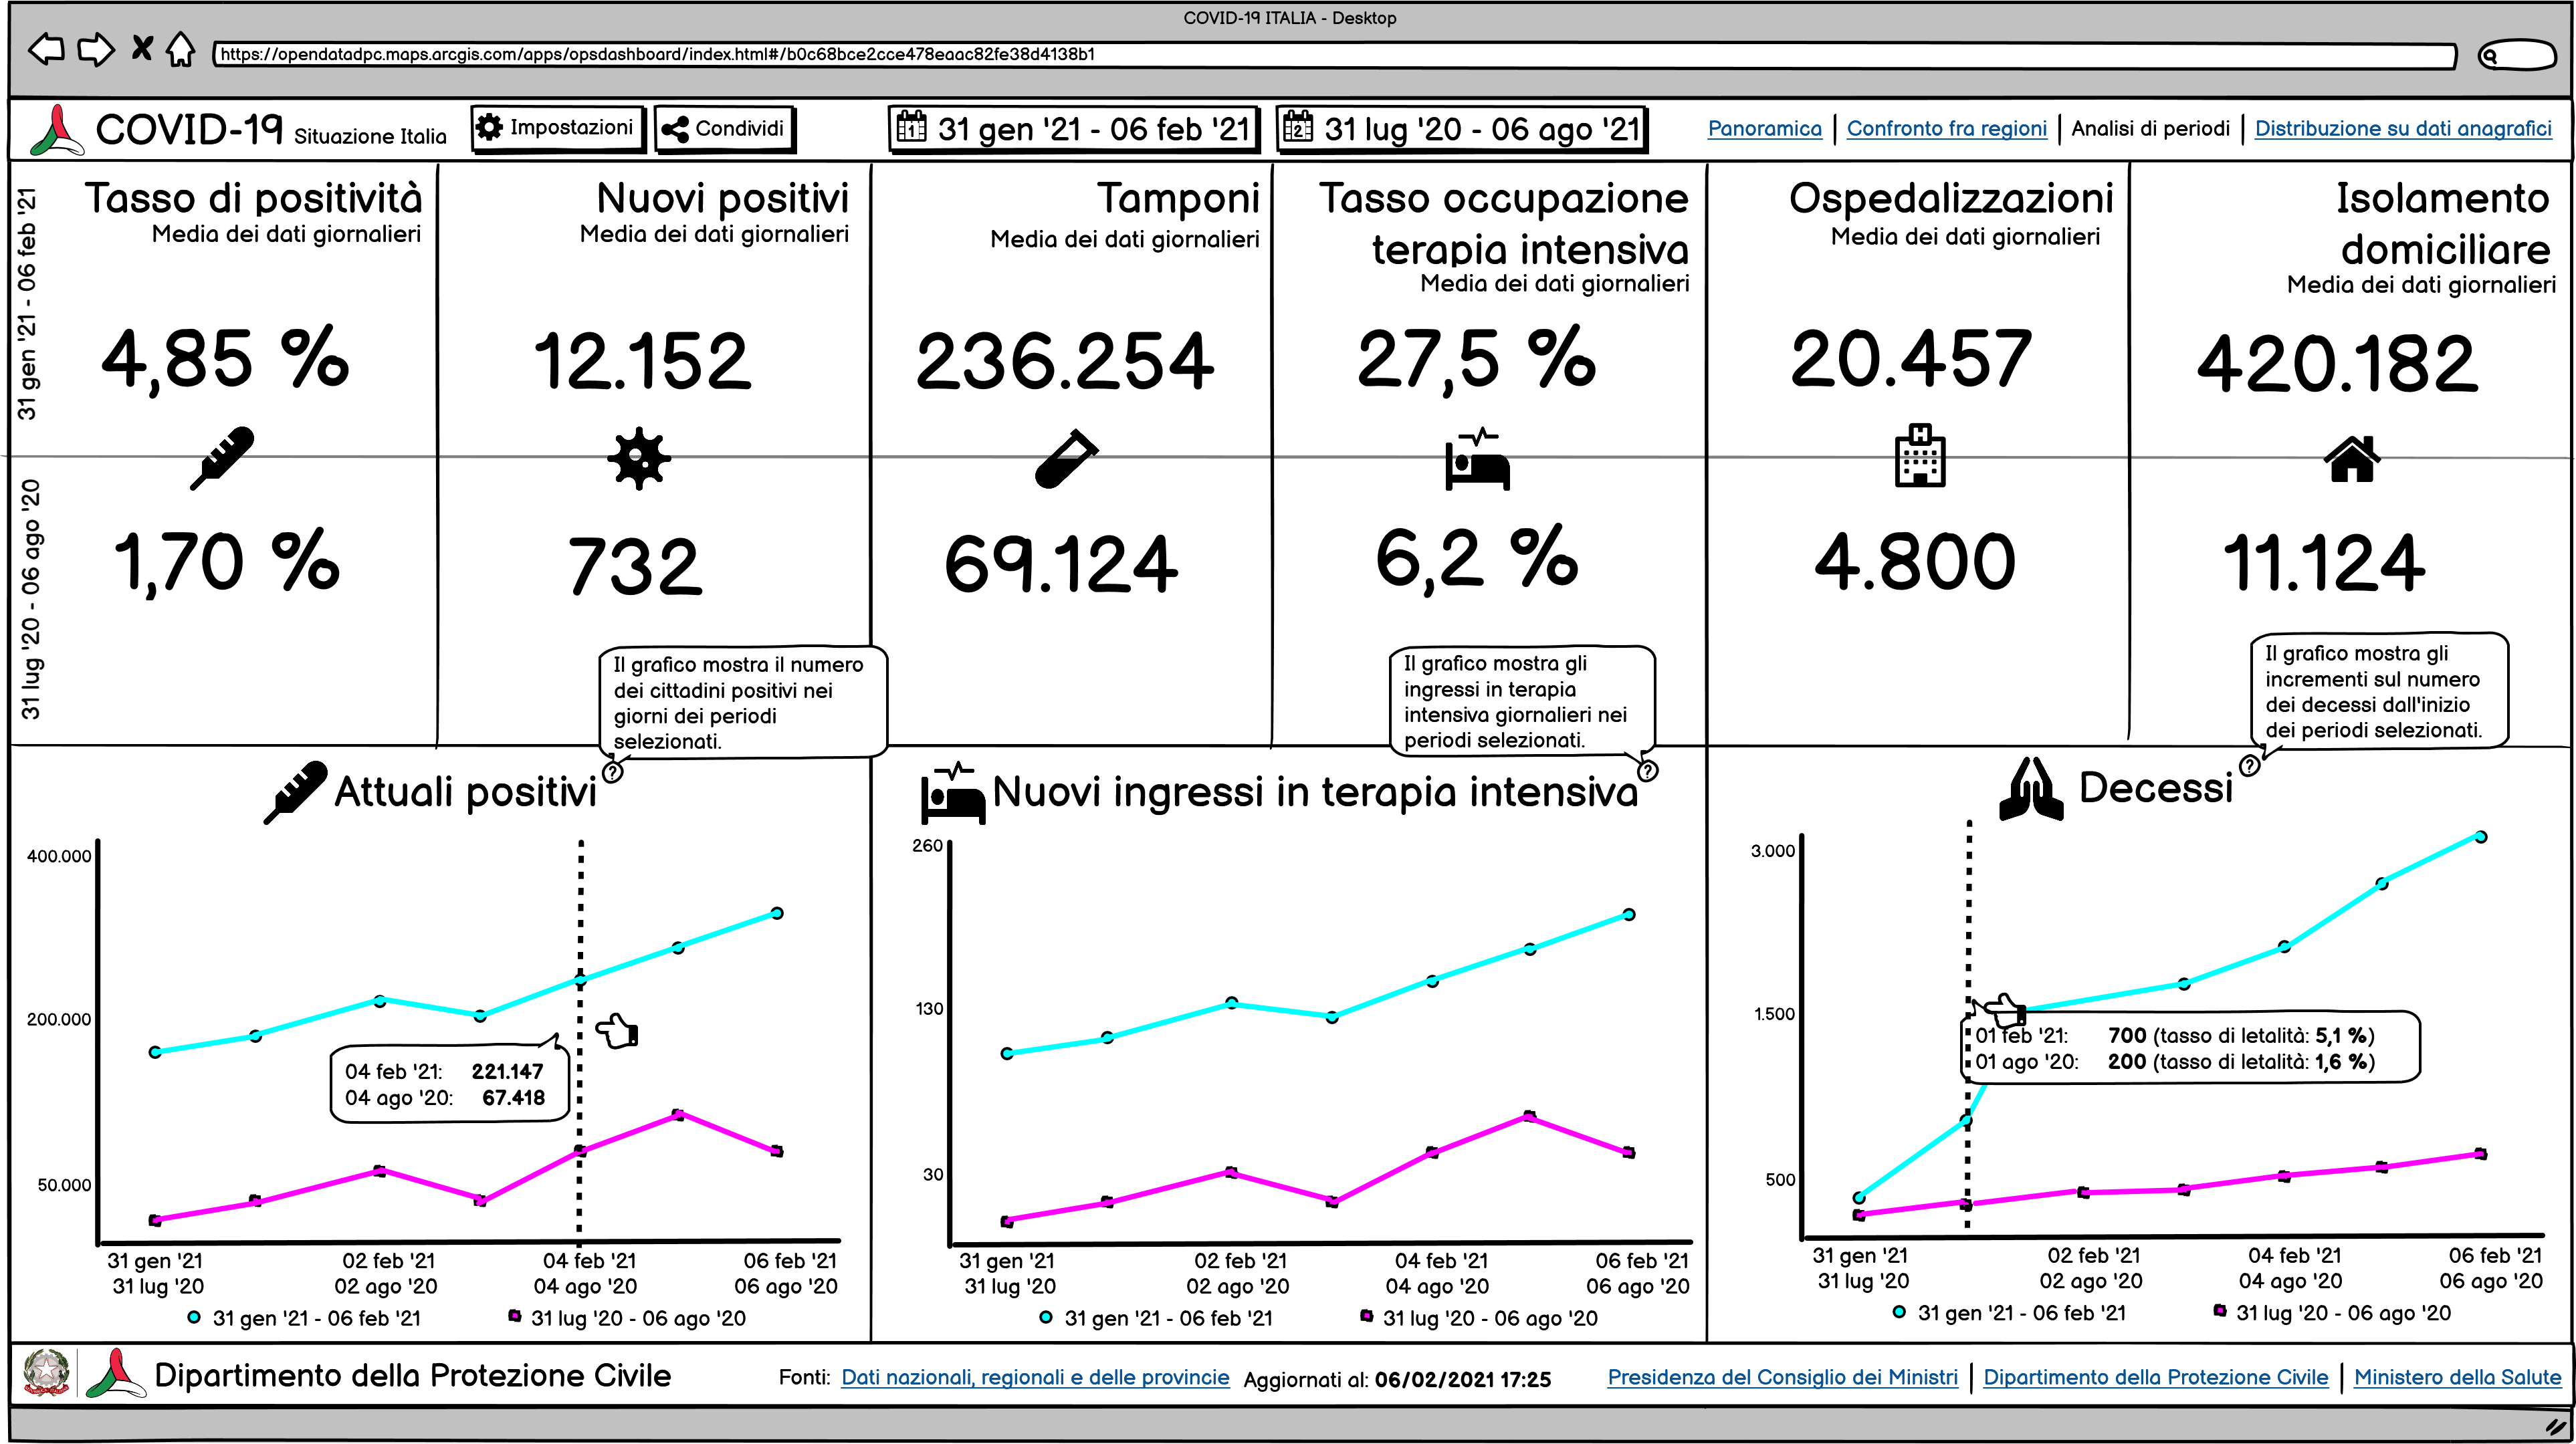
\includegraphics[width = \textwidth]{../img/1 - Analisi di periodi}
    \caption{Schermata "Analisi di periodi" dell'interfaccia riprogettata.}
    \label{fig:analisi-periodi}
\end{figure}
Questa schermata è di grande utilità per i giornalisti che vogliono analizzare l'andamento di certe metriche con riferimento ad uno o due periodi temporali.\\
Nella parte superiore, sono visualizzati i valori delle metriche aggregati sul o sui periodi temporali specificati, permettendo al giornalista di raffrontare immediatamente i valori stessi.\\
Nella parte inferiore, trovano spazio tre grafici che riportano gli andamenti delle metriche relativamente alla o alle finestre temporali fissate.

\clearpage
\subsection{Distribuzione su dati anagrafici}
\begin{figure}[h]
    \centering
    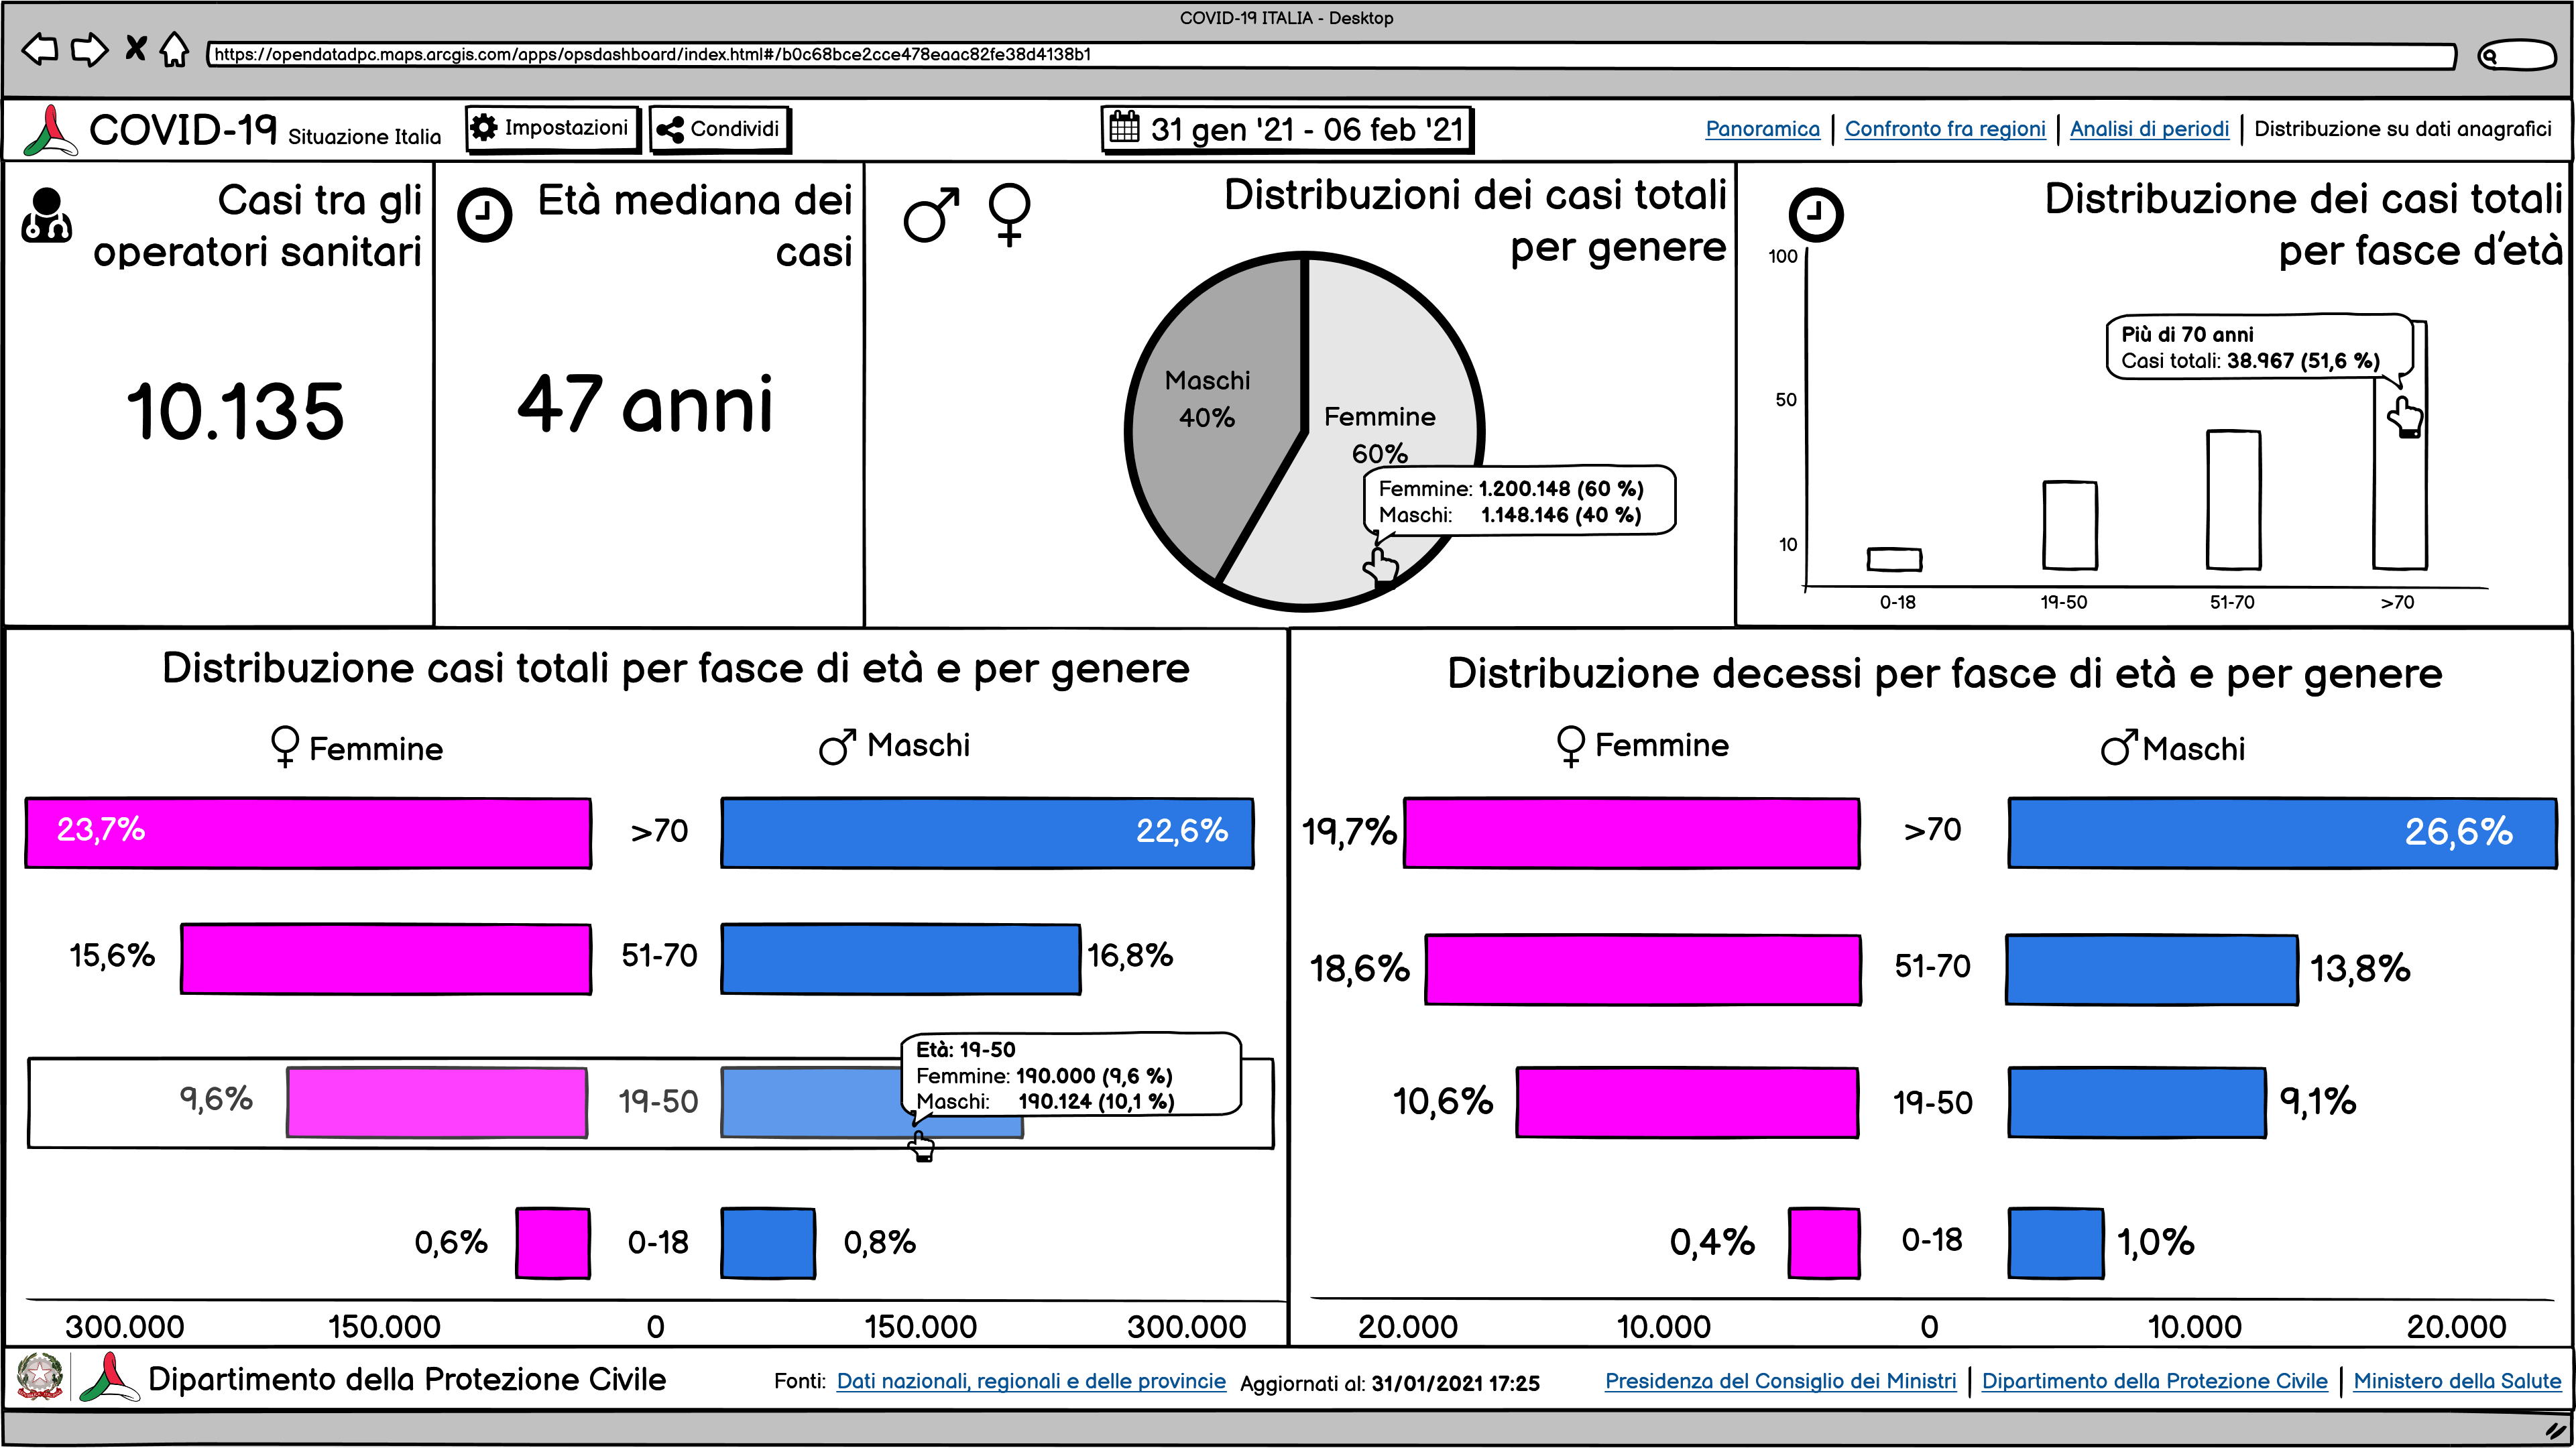
\includegraphics[width = \textwidth]{../img/1 - Distribuzione su dati anagrafici}
    \caption{Schermata "Distribuzione su dati anagrafici" dell'interfaccia riprogettata.}
    \label{fig:distribuzione-dati-anagrafici}
\end{figure}
La schermata in oggetto comunica ai giornalisti dati preziosi che permettono loro di comprendere la distribuzione delle metriche epidemiologiche rispetto a variabili anagrafiche, quali età, il genere e l'impiego.
In dettaglio, i giornalisti, nel momento in cui visitano questa schermata possono visualizzare e interagire con box numerici, grafici a barre e areogrammi, riuscendo a sviscerare, secondo eterogenee prospettive, le distribuzioni anagrafiche che intendono studiare.

\clearpage
\section{Risoluzione delle criticità}
Nella sezione corrente, elenchiamo la soluzione che abbiamo fornito per ogni criticità citata in \hyperref[ss:criticita]{Sezione 2.1 Criticità nell’esperienza utente}:
\begin{enumerate}
    \item [{\hyperref[el:1]{1.}}] abbiamo proceduto nella direzione di una migliore leggibilità del contenuto, ingrandendo la dimensione delle scritte particolarmente piccole e uniformando le dimensioni di tutte le componenti testuali in base alla loro importanza;
    \item [{\hyperref[el:2]{2.}}] abbiamo proceduto con l'analizzare l'importanza di ogni componente informativa, per poi mapparne la dimensione in maniera proporzionale: inoltre, abbiamo evitato la creazione di spazi vuoti, distribuendo tutti gli elementi in maniera omogenea sull'interfaccia; un esempio è la riprogettazione della componente che presenta le note, per la quale abbiamo cambiato il semplice box dell'interfaccia originale in una sidebar che compare al clic dell'utente su un bottone, con la conseguenza di dare maggiore spazio e leggibilità alle note stesse, senza sacrificare in maniera permanente lo spazio dell'interfaccia;
    \item [{\hyperref[el:3]{3.}}] abbiamo rivisto l'interazione offerta dalle mappe, cambiandone la natura da bubble map a heat map: in questa maniera, abbiamo semplificato per il giornalista la selezione di una certa regione, rendendola possibile cliccando semplicemente sull'area corrispondente;
    \item [{\hyperref[el:4]{4.}}] abbiamo proceduto col valutare l'interfaccia originale in termini di affordance\footnote{Per \textit{affordance} si intendono quelle proprietà degli oggetti che forniscono suggerimenti sul come utilizzarli.} e significanti, al fine di disambiguare ogni possibile interazione: ad esempio, i bottoni sono chiaramente caratterizzati e al loro click seguono sempre azioni e/o feedback inequivocabili, mentre i vari elementi delle mappe e delle tabelle reagiscono al passaggio del cursore suggerendo la loro natura interattiva;
    \item [{\hyperref[el:5]{5.}}] abbiamo migliorato l'usabilità del widget calendario, nonché adottato alcuni accorgimenti per prevenire o ridurre errori accidentali del giornalista: un esempio è l'aver disabilitato le date successive al giorno corrente, impedendo al giornalista di selezionare così date per cui la dashboard non visualizzerebbe valori; inoltre abbiamo aggiunto dei bottoni tramite cui l'utente può agevolmente andare al giorno successivo o precedente a quello selezionato o, ancora, resettare la selezione alla data corrente;
    \item [{\hyperref[el:6]{6.}}] abbiamo aggiunto nuove funzionalità alla mappa, sotto forma di bottoni al cui clic l'utente può resettare il livello di zoom a quello di default o centrare la porzione visualizzata sulla sua posizione effettiva mediante geolocalizzazione; 
    \item [{\hyperref[el:7]{7.}}] trasversalmente alle schermate dell'interfaccia riprogettata, abbiamo aggiunto icone al fine di ridurre il carico cognitivo richiesto al giornalista per individuare e distinguere le varie componenti informative;
    \item [{\hyperref[el:8]{8.}}] abbiamo ridotto l'utilizzo del colore come elemento distintivo delle componenti, affiancandolo piuttosto sempre ad almeno un ausilio addizionale: esempi sono il diverso tratto delle curve dei grafici, nonché la sottolineatura dei link;
    \item [{\hyperref[el:9]{9.}}] abbiamo semplificato l'interazione coi grafici, facendo sì che al movimento del cursore corrisponda una proiezione sull'asse delle $x$ che intercetti le curve: in questa maniera, il giornalista può ottenere i dati puntuali, in maniera semplice, ponendo il cursore in un qualsiasi punto soprastante o sottostante a quello di suo interesse; 
\end{enumerate}
	
Ulteriormente, abbiamo aggiunto funzionalità nuove che, stando alle dichiarazioni dei giornalisti, permettono un'usabilità, esperienza d'uso e utilità superiori.\\
Tra queste, da annoverare è la personalizzazione del contenuto informativo delle diverse componenti di ogni schermata; in dettaglio, nell'intestazione delle schermate abbiamo inserito un bottone chiamato "Impostazioni", al cui clic compare la lista delle metriche disponibili per la schermata corrente, ognuna delle quali può essere trascinata all'interno della schermata stessa, in sostituzione di una componente preesistente. Abbiamo pensato a questa funzionalità con l'obiettivo di fornire quanta più informazione al giornalista senza sacrificarne la leggibilità.

Altra funzionalità aggiunta è la comparsa a schermo di pop-up informativi per avvisare il giornalista del caricamento dei nuovi dati del giorno corrente: dal momento che, quotidianamente, i nuovi dati sono resi disponibili nella fascia oraria che va dalle 17 alle 19, ecco che l'utente può aprire la dashboard alle 17 e continuare i propri task tranquillamente, senza dover continuamente riaggiornarla per capire se i dati sono giunti, consapevole che sarà avvisato prontamente dal pop-up.

\end{document}
